
%\documentclass[letterpaper, 10 pt, conference]{ieeeconf}  % Comment this line out
                                                          % if you need a4paper
\documentclass[a4paper, 10pt, conference]{ieeeconf}      % Use this line for a4
\usepackage[pdftex]{graphicx}

%%% LITTERATURLISTE %%%
\usepackage[square,numbers]{natbib}
\usepackage{url}

                                                          % paper

% \IEEEoverridecommandlockouts                              % This command is only
                                                          % needed if you want to
                                                          % use the \thanks command
% \overrideIEEEmargins
% See the \addtolength command later in the file to balance the column lengths
% on the last page of the document

\title{\LARGE \bf
Totally Awesome Title That Will Totally Look Good Even Though It is Long
}


\author{Morten Moeller Jakobsen, Casper Holst Laustsen and Johan Leth Gregersen% <-this % stops a space
\thanks{*This work was not supported by any organization}% <-this % stops a space
\thanks{*The Department of Computer S, Aalborg University}%
}



\begin{document}



\maketitle
\thispagestyle{empty}
\pagestyle{empty}


%%%%%%%%%%%%%%%%%%%%%%%%%%%%%%%%%%%%%%%%%%%%%%%%%%%%%%%%%%%%%%%%%%%%%%%%%%%%%%%%

\begin{abstract}

This electronic document is a ÒliveÓ template. The various components of your paper [title, text, heads, etc.] are already defined on the style sheet, as illustrated by the portions given in this document.

\end{abstract}

%%%%%%%%%%%%%%%%%%%%%%%%%%%%%%%%%%%%%%%%%%%%%%%%%%%%%%%%%%%%%%%%%%%%%%%%%%%%%%%%
\section{INTRODUCTION}
\label{sec:intro}

The rising interest, research and development of GPS devices, have increased potential market significantly. With cheaper devices comes a larger number of potential applications. Having constant feeds of GPS coordinates of the vehicle network in real-time with high accuracy gives the market some unique feats that makes it interesting for a broader spectrum of companies.

Insurance companies are one of the newer additions to this spectrum of companies. Car insurances has traditionally been based on the facts available at the time of purchase. Insurance companies will usually require detailed information about you and your car, creating an offer based on that. Coupled with historical statistics, an insurance company can make reasonable predictions about risks associated with insuring your car. For example, statistics often show young drivers being involved in more accidents compared to others\cite{accidents}.

Basing insurance on such loose prediction criteria is unfair for the individual policy holder. The generalization that young people are bad drivers means that even those who drive very well, have to pay extra because of those who do not. The problem is not unrecognised, and it is also being addressed by both insurance companies and researchers (See \ref{sec:RelatedWork}).

Insurance companies have always had historical data of what makes a driver more likely to be a poor driver. Looking at this data will clearly state different trends\cite{url:forbes}, e.g. driving at friday or saturday nights, or being young will make you more likely to be participant in an accident. Real-time data feeds offers a lot of information, such as the customers driving patterns, e.g. how steady speed the customer often has, how often he is speeding or even how often he hard he normally brakes.

To make insurance fairer, it makes sense to look at individuals rather than segmented groups. If risk prediction could be calculated based on the use of individual cars, that also means the policy holder could receive a fair price offer. This type of insurance is known as Usage Based Insurance (UBI) or Pay-As-You-Drive(PAYD), and a few insurance companies is already offering it as a product. By example, the American company \texttt{Progressive} sells UBI in select states under the name \texttt{Snapshot}\cite{snapshot}. The insurance depends on their own device mounted in your cars OBD-II port, which then measures how much you drive, number of hard braking events and more.

A common factor for any UBI system is the requirement for certain hardware in insured cars. The insurance company needs data, which the device must provide. The data is usually sent directly from the device to the insurance company, which is also the case in before mentioned example. This model can however be a concern for the policy holder. The data can be inaccessible, since it is sent directly to the insurance company. It then depends on the insurance company which data the policy holder can see, and it might not be possible to verify if you are being billed correctly. Furthermore, it is not transparent which data the insurance company actually has on your car. In Progressive's example it can be read from their FAQ that "some devices collect location data", which may be a privacy concern, especially given that the data can not be accessed.

In this paper the authors suggest how to alleviate concerns of the policy holder, while still maintaining a logical model that works for the insurance company. The data warehouse has to been implemented with a efficient and easy querying in mind. The authors look into which data is needed by the insurance company, and how it can be sent to them without being able to track policy holders too closely. There is a presentation of a series of metrics, made possible through collected vehicle data, and provide intuitive ways to visualize them for the policy holder.

The main challenges in achieving these goals lies in data management, both for supporting different metrics, but also for privacy-friendly alteration. Data presentation is also a significant challenge, as raw log data will have to be displayed in a way that the policy holder can relate and understand.


\section{DATA FOUNDATION}\label{sec:datafound}

This section describes the different data sources. The first paragraph describes concepts that are vital for the understanding of this paper.
The paragraphs after describe the basis data foundation for the system, namely the INFATI dataset and OpenStreetMap.

\subsection{Preliminary Concepts}\label{subsec:precon}
\textbf{Metrics} is a set of attributes describing the way a car travels from a position  to a destination. Measures are calculated point by point in a GPS Fact, and a point describes what has changed since the previous point. The chosen metrics are metersdriven(meters), critical time(high risk temporal timespan), roadtype(high risk spatial segments), acceleration($m/s^2$), brake($m/s^2$), jerk($m/s^3$), meters sped(meters), steady-speed(boolean). 

\textbf{Policy} is a billing scheme for an insurance company. Given this scheme, the cost of a given set of metrics for a trip is defined. If the policy is changed, the cost of a trip is changed. An insurance company have the option to run multiple policies.

\textbf{Trips} are the authors term for set of continual GPS-coordinates. Whenever 3 minutes passes after the last GPS-point was logged, the trip is ended. The next GPS-point logged will be the starting point of the next trip. Trips should not be mistaken for a tripfact, which will be explained later.

\subsection{INFATI dataset}
The INFATI dataset\cite{art:INFATI} is a collection of spatio-temporal data, collected in 2000-2001. It consist of 20 unique cars, each providing their own separated collection of data. This is a total of 1.895.085 rows of spatio-temporal car-data. The data is logged with 1Hz, and mainly involves trajectories in northern Jutland. The purpose of the INFATI\cite{art:INFATI} project was to research driver response to alert issued by a device installed in the car. A green light is shown when the car is below the speed limit. A red light is displayed when above the speed limit, additional to a womans voice saying ''you are driving too fast''.

\subsection{OpenStreetMap}
OpenStreetMap\cite{osm} is a an open source digital roadmap offered  and maintained by the OpenStreetMap community. This project makes use of the digital roadmap of Denmark, which was provided along-side the INFATI dataset\cite{art:INFATI}. The digital roadmap of Denmark contains 762.155 rows of segment information.

\section{LOGICAL MODEL STRUCTURE}\label{sec:dataware}

The logical model of the data warehouse is a snowflake schema as shown in Figure \ref{fig:datawarehouse}. It consists of a total amount of 8 different tables, 3 of those being fact tables. Trivial dimensions like Date and Time will not be described in depth. The color encoding is as following; Purple entities are exclusively on the clients side, the red entities are on both the clients side and the insurance companys side. The green entity is implemented on the client side, and has special situational relation to the insurance company, which will be described in depth in the next paragraph.

\begin{figure*}[tb]
\centering
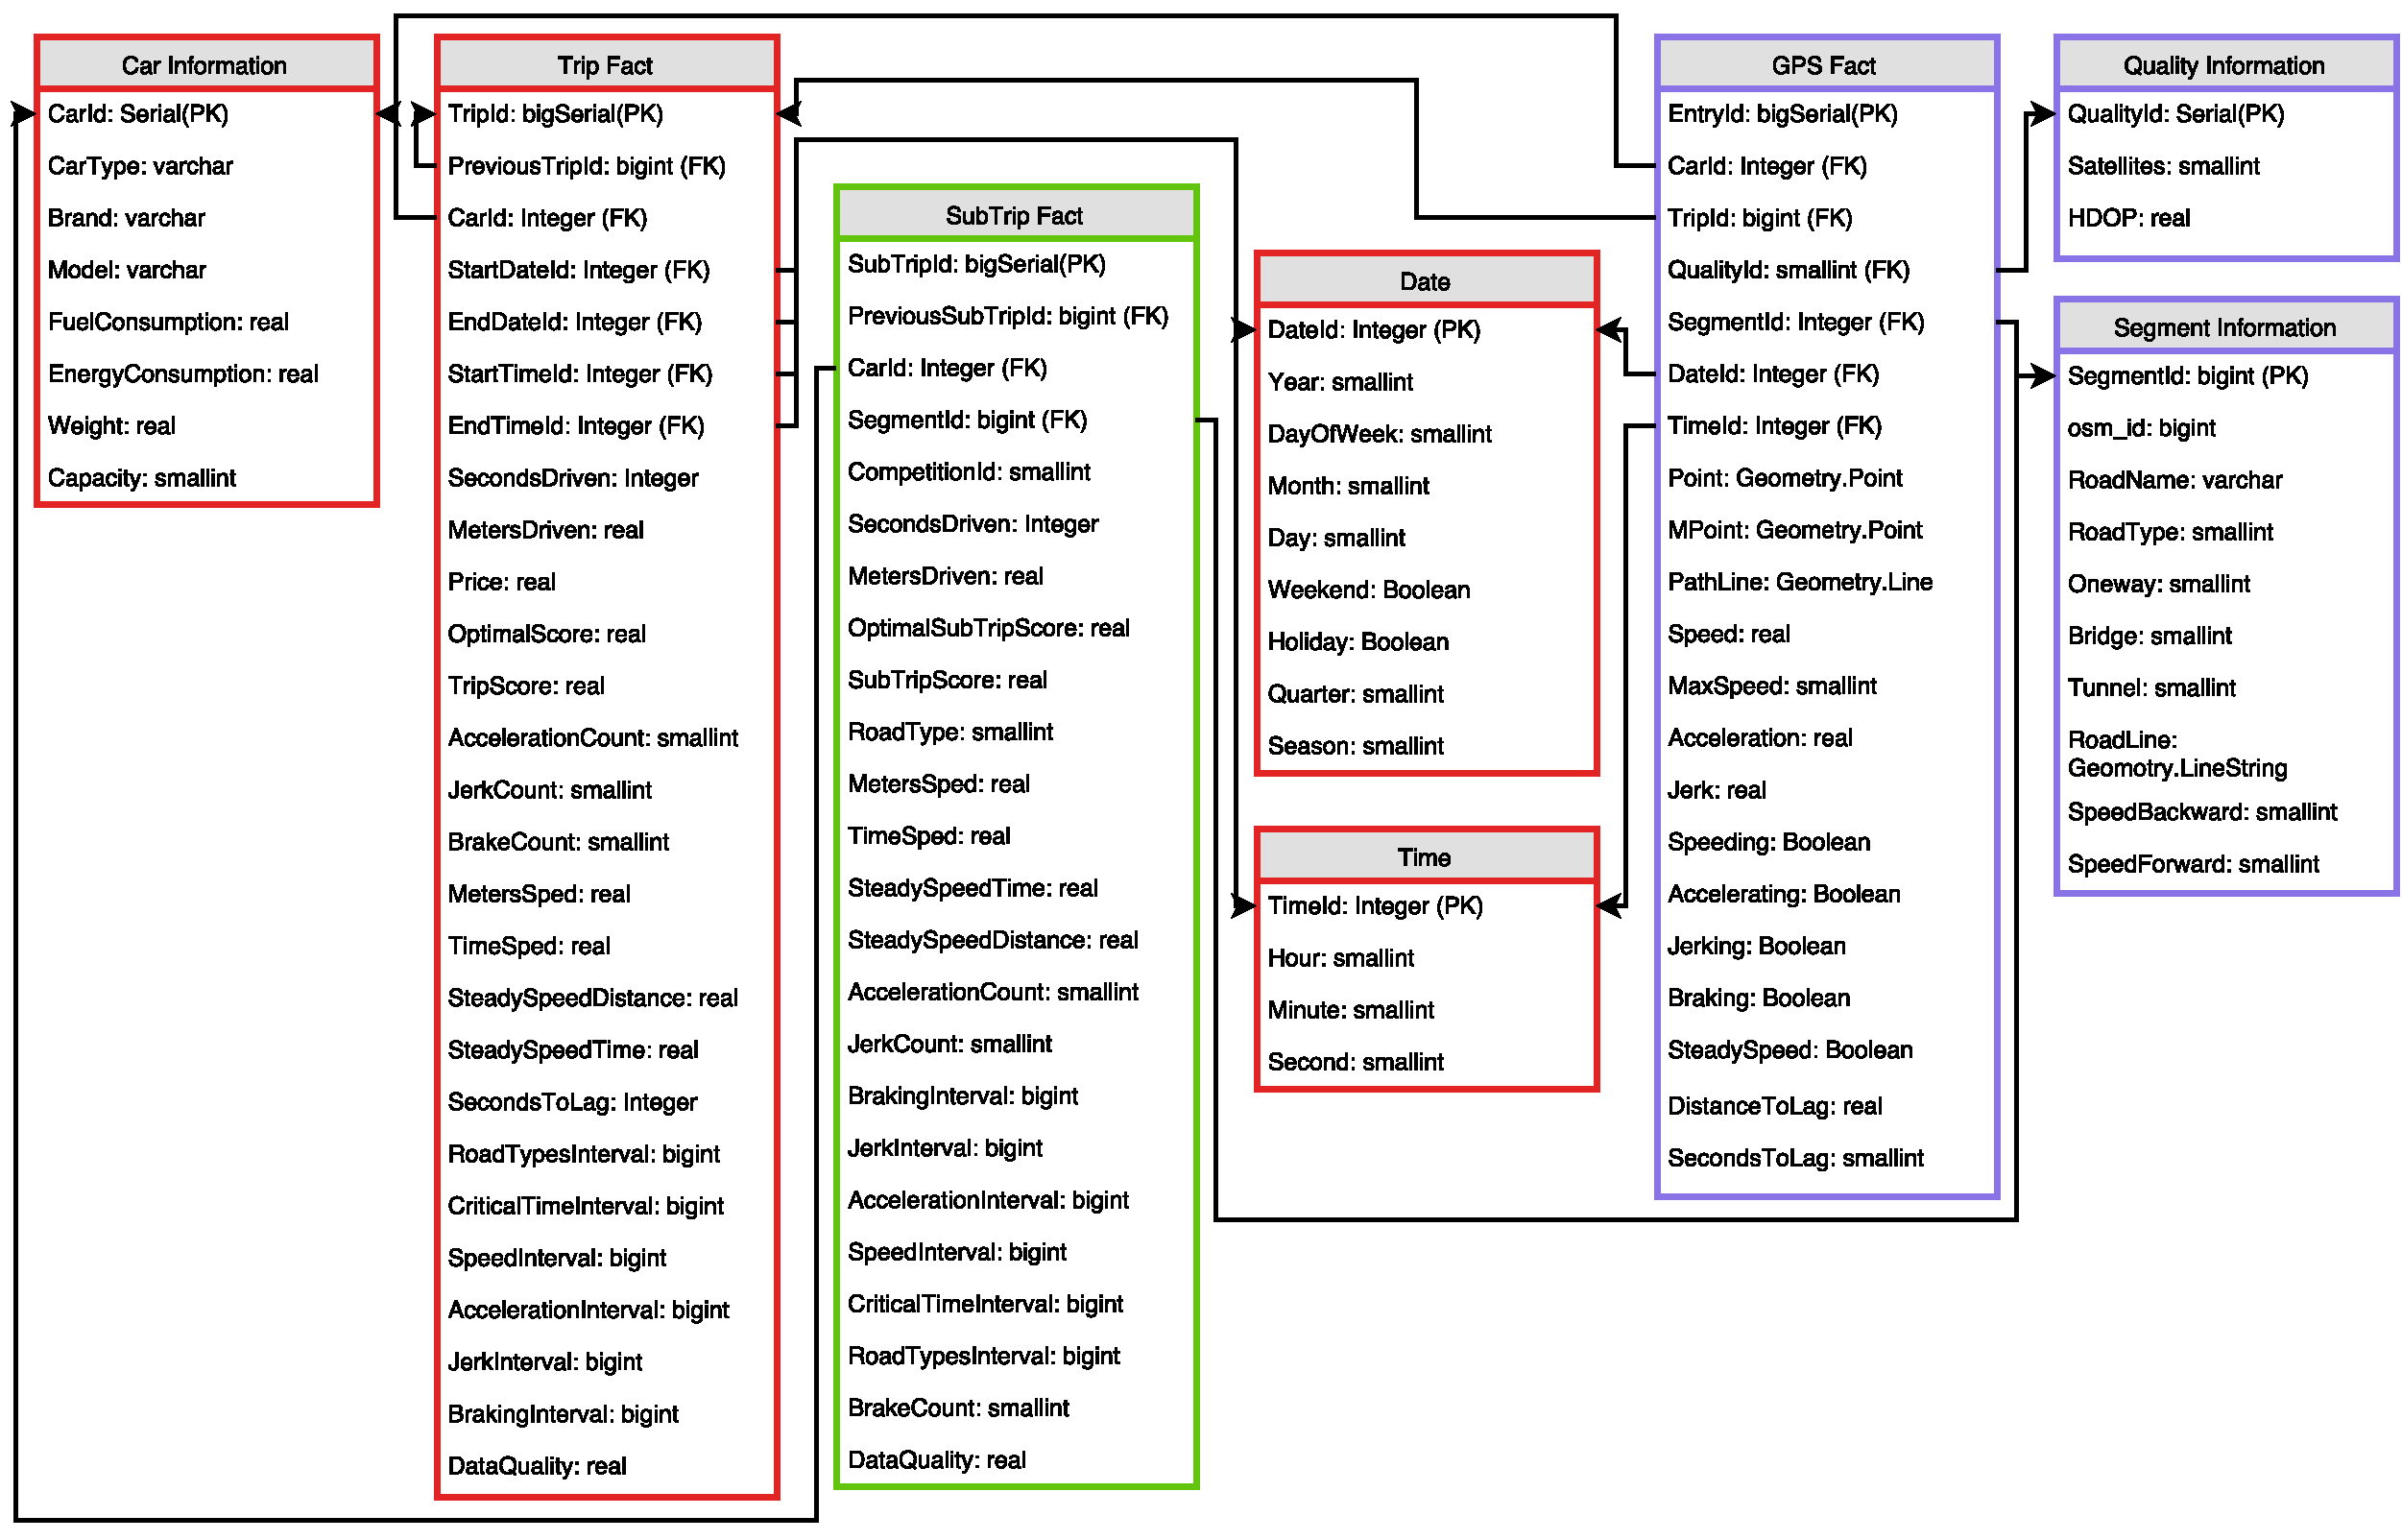
\includegraphics[width=0.9\textwidth]{Pictures/ERDiagram}
\caption{Logical Model of the Data Warehouse}
\label{fig:datawarehouse}
\end{figure*}

\subsection{Fact Tables}

Amongst the fact tables there is a certain hierarchy, the GPS fact table is the main fact table where each entry is logged through the logging device. Certain values are calculated on the logged entry, and added to the database. After the journey has ended, a tripfact is then calculated given the gpsfacts. Subtripfacts are calculated from the gpsfacts associated with each segmentid in the journey. The interaction will be further described in \nameref{sec:ETL}.

\textbf{GPS Fact} is the center of the entire data warehouse. Each entry represents a singular GPS point of a car, with the actual timestamps. The table references all of the support tables, as well as a reference to a single tripfact. A GPS fact contains spatial attributes in \textit{Point},\textit{MPoint} and \textit{PathLine}, being GPS coordinates, map-matched GPS coordinates and a line from the previous GPS coordinate respectively. A gpsfact contains multiple Booleans, namely \textit{Speeding}, \textit{Accelerating}, \textit{Jerking}, \textit{Braking} and \textit{SteadySpeed}, which are primarily added for query-facilitation as the actual value exists in different attributes. The actual values of the attributes are all calculated in relation to the previous points e.g. acceleration is the change in speed between now and previous point divided by the distance between them.

\textbf{Trip Fact} entries represents an actual car trip through a sample of GPS coordinates. They contain a start-time and an end-time represented by 4 foreign keys to the Date and Time dimensions. A tripfact has a lot of attributes which is simply an addition from the sample of gpsfacts, namely \textit{MetersDriven}, \textit{SecondsDriven} and all of the count attributes. Each trip fact has a \textit{TripScore} and \textit{OptimalScore} which is the calculated based on the insurance policy used, this will be described later in \ref{sec:trip}. A contribution of this article is the decision to create intervals in the form of a bigint, to represent to which degree an actual delinquency is. To explain this further, here is a clean example in Table \ref{tab:intervalexampe} with Acceleration; 

\begin{table}[h]
\centering
\begin{tabular}{cc | cc}
\multicolumn{2}{c}{\textbf{Policies}} & \multicolumn{2}{c}{\textbf{Logged Info}} \\\hline
\textbf{Intervals ($m/s^{2}$)}     & \textbf{Weights}     & \textbf{Delinquencies}     & \textbf{Percentage}     \\\hline
{[}3, 4 {[}              & 1.05              &   32            & 40              \\
{[}4, 4.5 {[}            & 1.10              &   16            & 20              \\
{[}4.5, 5 {[}            & 1.15              &   8             & 10              \\
{[}5, 5.5 {[}            & 1.25              &   4             & 5              \\
{[}5.5, 6 {[}            & 1.35              &   8             & 10              \\
{[}6, 6.5 {[}            & 1.45              &   4             & 5              \\
{[}6.5, 7 {[}            & 1.55              &   8             & 10              \\
{[}7, $\infty$ {]}       & 1.80              &   0             & 0              \\\hline
\end{tabular}
\caption{An example of Acceleration Interval}
\label{tab:intervalexampe}
\end{table}

All of the accelerations for the trip are divided into different intervals depending on their severity. The intervals and weights are determined by some policy presented by the insurance company, meaning you can have different policies throughout the system. The policy is represented by the 2nd and 3rd digit in the bigint. As the total amount of delinquencies can extend 100, and there is only 2 digits representing each number, the percentage of delinquencies are used instead. If one of the intervals contains 100\% of the delinquencies, the 1st digit of the bigint is set to 1. So this particular example would result in the following interval representation in bigint;

$$
0\ 01\ 32\ 16\ 08\ 04\ 08\ 04\ 08\ 00 \eqno{(1)}
$$
given a policy with id 1.

\textbf{SubTrip Fact} is a special fact table in the sense that it does not have any direct impact on the insurance. It is created with gamification in mind, making it possible to compare different clients and their driving-patterns to each other on certain segments. Direct comparison between full tripfacts are hard because the routes are quite unique. Aside from only covering a certain segment, the SubTrip Fact table is very similar to the Trip Fact. One of the more noticable differences however are the fact that a subtripfact has a \textit{competitionId}, which makes it possible for the insurance company to create competitions on certain segments.


\subsection{Information Tables}

\textbf{Car Information} is a support table holding valid information about the user's car. The data is valuable to the insurance company, if not for actual insurance calculations, then for statistical use. The data is of a relation 1 to many tripfacts, subtripfacts or gpsfacts, meaning each of these fact tables must have a link to an entry in Car Information. This is important because an insurance policy  is per car rather than per person.

\textbf{Quality Information} is a support table which determines the quality of the given gpsfact. The table contains information on the Horizontal-Dilution-of-Position(HDOP) and the amount of satellites covering the car. Whenever the algorithm encounters a new unseen combination of the two, it creates an entry in the database. Entries are mapped 1 to many gpsfacts because of this, but  the amount of duplicated information is reduced.

\textbf{Segment Information} is the last support table and it has the entire road network of Denmark from OpenStreetMap\cite{osm}. The osm\_id is kept to make it possible for cooperation and better integration in the future. Segment Information is related 1 to many to both subtripfacts and gpsfacts.

\section{ETL}\label{sec:ETL}
The data foundation for this project relies on two sources, refer section \ref{sec:datafound}. ETL is an important phase to integrate these two sources of information into the data warehouse while ensuring a uniform data-representation. A preprocessing procedure fills static support-tables and dimensions with data. The data foundation contains data for car information and part of GPS Fact. After the preliminary data is loaded, a number of post-processing procedures fills the remaining tables in the data warehouse with data.

The INFATI project\cite{art:INFATI} uses a digital roadmap from OpenStreetMap\cite{osm}. The same digital roadmap is used for this project. A few modifications is introduced, like storing the column \textit{direction} as a smallint instead of a textual representation. 

The INFATI dataset\cite{art:INFATI} contais 17 columns of data, separated by a varying number of spaces. Due to the natural challenges of map-matching, some entries contain only 14 columns of data. This cause the dataset to have problems with trailing zeros when loading with a space-separator. To ease the ETL process, a script is made to alter the separator into a \#. Whenever a row was not map-matched, three \#'s is appended to that row.

INFATI coordinate-sets are stored in Universal Transverse Mercator (UTM 32) format. This system is build on GPS, and a transformation from UTM to lattitude and longitude is needed. Coordinate-sets are stored as points, lines or polygons and stored in the data warehouse as PostGIS\cite{postgis} geometries. These geometries has to be assigned the correct spatial reference system identifier(SRID), otherwise they will refer to an incorrect positions. INFATI is logged in UTM32 North format, which has SRID 23032\cite{UTM32N}. Latitude and Longitude format is part of World Geodetic System(WGS), namely WGS84, and has SRID 4326\cite{WGS84}. To transform the format: the geometry is created, assigned the UTM SRID, and transformed into WGS84 latitude longitude format using WGS84 SRID. 

Appropriate data for the support-table: Quality Information and dimensions: Date and Time are computed and stored.

The preprocessing is now complete, and the INFATI data can be loaded into the data warehouse. A car must be created and stored in Car Information-table, hereafter the corresponding INFATI-data is loaded into the GPS Fact-table. 

The postprocessing will now begin with dividing the batch of gpsfacts into trips for each car. Each found trip will be stored in the Trip Fact by a TripId and corresponding CarId, and the entire GPSFact-table will be updated for TripIds. 

GPS Fact measures will then be calculated for all trips and cars. The process will take one car at a time, fetch all TripIds for that car, go over each trip and compute measures, update the gpsfacts with these measures.

When the GPS Fact is updated with measures, it is possible to compute the measures for the Trip Fact-table. The process will take one car at a time, fetch all TripIds for that car, go by one trip at a time and fetch all gpsfacts for that trip. Whenever the measures has been calculated for a given trip, the Trip Fact is updated.

SubTrip Fact is only conceptual at this time. It is not calculated and stored in the data warehouse. Though, it would primarily use the same computations as TripFact which would make this process relatively trivial.

Given a working setting for the system, it could be another data-representation that the system would receive. This calls for designing and coding another ETL-procedure that will transform this data into the uniform data-representation present in the data warehouse.

%Måske skal det her ikke med?
To decrease the computation-time of the ETL-phase, the loading-process has been multi-threaded so that a single car is being loaded in its individual thread. This is only relevant for the INFATI dataset. In a working setting, data would come in bulks of single trips. 

\section{TRIP SCORING}\label{sec:trip}

Before you begin to format your paper, first write and save the content as a separate text file. Keep your text and graphic files separate until after the text has been formatted and styled. Do not use hard tabs, and limit use of hard returns to only one return at the end of a paragraph. Do not add any kind of pagination anywhere in the paper. Do not number text heads-the template will do that for you.

Finally, complete content and organizational editing before formatting. Please take note of the following items when proofreading spelling and grammar:

\subsection{Subscores} Define abbreviations and acronyms the first time they are used in the text, even after they have been defined in the abstract. Abbreviations such as IEEE, SI, MKS, CGS, sc, dc, and rms do not have to be defined. Do not use abbreviations in the title or heads unless they are unavoidable.

\subsection{Calculating Trip Scores}

\begin{itemize}

\item Use either SI (MKS) or CGS as primary units. (SI units are encouraged.) English units may be used as secondary units (in parentheses). An exception would be the use of English units as identifiers in trade, such as Ò3.5-inch disk driveÓ.
\item Avoid combining SI and CGS units, such as current in amperes and magnetic field in oersteds. This often leads to confusion because equations do not balance dimensionally. If you must use mixed units, clearly state the units for each quantity that you use in an equation.
\item Do not mix complete spellings and abbreviations of units: ÒWb/m2Ó or Òwebers per square meterÓ, not Òwebers/m2Ó.  Spell out units when they appear in text: Ò. . . a few henriesÓ, not Ò. . . a few HÓ.
\item Use a zero before decimal points: Ò0.25Ó, not Ò.25Ó. Use Òcm3Ó, not ÒccÓ. (bullet list)

\end{itemize}


\section{EXPERIMENTS}\label{sec:expe}
The main focus of the experiments section is to demonstrate the trip scoring. Primarily to demonstrate the possibility to score similar routes differently, based on the calculated metrics stored in the system. Therefore, a policy is created using parameters and variables found reasonable by the authors. An insurance company would have to decide on these parameters for policies offered to customers. The chosen parameters and values can be seen in the tables \ref{tab:roadtypevalues}, \ref{tab:crittimevalues}, \ref{tab:speedingvalues}, \ref{tab:accelerationvalues}, \ref{tab:basevalues}, and \ref{tab:polyvalues}.

\begin{table}
    \centering
    \begin{tabular}{ll}
    \textbf{Roadtype} & \textbf{Weight} \\ \hline
    Motorway          & 1               \\
    Trunk             & 1               \\
    Primary           & 1               \\
    Secondary         & 1.05            \\
    Tertiary          & 1.1             \\
    Unclassified      & 1.1             \\
    Residential       & 1.2             \\
    Service           & 1.2             \\ \hline
    \end{tabular}
    \caption{Roadtypes with weights}
    \label{tab:roadtypevalues}
\end{table}

\begin{table}
    \centering
    \begin{tabular}{llll}
    \textbf{Active days} & \textbf{Start} & \textbf{End} & \textbf{Weight} \\ \hline
    Monday - Friday      & 07:00:00       & 09:00:00     & 1.2             \\
    Monday - Friday      & 15:00:00       & 17:00:00     & 1.15            \\
    Saturday - Sunday    & 09:00:00       & 13:00:00     & 1.025           \\
    Saturday - Sunday    & 20:00:00       & 23:59:59     & 1.15            \\
    Saturday - Sunday    & 00:00:00       & 00:04:00     & 1.4             \\ \hline
    \end{tabular}
    \caption{Critical time intervals with weights}
    \label{tab:crittimevalues}
\end{table}

\begin{table}
    \centering
    \begin{tabular}{ll}
    \textbf{Interval (\%)}   & \textbf{Weight} \\ \hline
    {[}0, 10{[}        & 1.3                   \\
    {[}10, 20{[}       & 1.4                   \\
    {[}20, 30{[}       & 1.5                   \\
    {[}30, 40{[}       & 1.6                   \\
    {[}40, 50{[}       & 1.7                   \\
    {[}50, 60{[}       & 1.8                   \\
    {[}60, 70{[}       & 1.9                   \\
    {[}70, $\infty${]} & 2                     \\ \hline
    \end{tabular}
    \caption{Speeding intervals with weights}
    \label{tab:speedingvalues}
\end{table}

\begin{table}
    \centering
    \begin{tabular}{ll}
    \textbf{Interval (m/s)} & \textbf{Weight} \\ \hline
    {[}0, 3{[}              & 1               \\
    {[}3, 5{[}              & 1               \\
    {[}5, 7{[}              & 1.075           \\
    {[}7, 8{[}              & 1.1             \\
    {[}8, 9{[}              & 1.2             \\
    {[}9, 10{[}             & 1.4             \\
    {[}10, 11{[}            & 1.6             \\
    {[}11, $\infty${]}      & 1.9             \\ \hline
    \end{tabular}
    \caption{Acceleration, brake and jerk intervals with weights}
    \label{tab:accelerationvalues}
\end{table}

\begin{table}
    \centering
    \begin{tabular}{ll}
    \textbf{Action} & \textbf{Base weight} \\ \hline
    Acceleration    & 50                   \\
    Brake           & 75                   \\
    Jerk            & 62.5                 \\ \hline
    \end{tabular}
    \caption{Base weights for accelerations, brakes and jerks}
    \label{tab:basevalues}
\end{table}

\begin{table}
    \centering
    \begin{tabular}{ll}
    \textbf{Parameter} & \textbf{Weight} \\ \hline
    A                  & 1.02            \\
    B                  & 1.05            \\
    C                  & 0               \\
    Polynomial degree  & 1.08            \\ \hline
    \end{tabular}
    \caption{Weights for all polynomial functions}
    \label{tab:polyvalues}
\end{table}

To test this policy, and thereby the developed scoring system, trips were handpicked from the INFATI dataset\cite{art:INFATI}. This was done on the following criteria:

\begin{itemize}
  \item Trips should follow similar routes
  \item Trips should be similar in distance
  \item Trips should display different driving styles
\end{itemize}

From these criteria, two different test cases were picked. The trips included in these cases are visualized in figures \ref{fig:shorttrips} and \ref{fig:longtrips} with two and three trips respectively. The first being two short-distance trips, and second being three long-distance trips.

\subsection{Experiment 1: Short trips} \label{subsec:expe1}
The trips chosen for experiment 1 are visualized in Figure \ref{fig:shorttrips} and represents two $\sim$8.1km trips with a similar route. They are driven back and forth with the same car, on the same day. The route driven is simple and has very few turns. The trips are visualized using a green and red color.

\begin{figure}[tb]
    \centering
    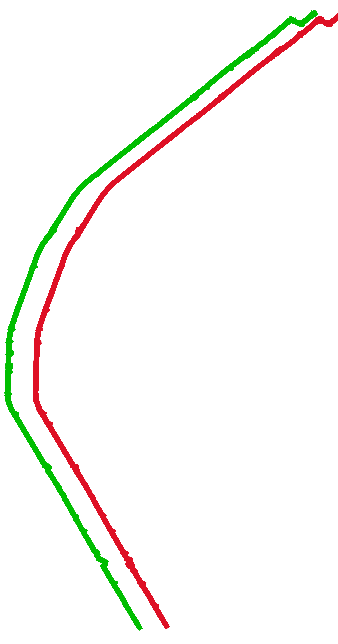
\includegraphics[width=40mm]{Pictures/ShortTrips.png}
    \caption{Green and red route for experiment 1}
    \label{fig:shorttrips}
\end{figure}

For naive usage-based-insurance, the car owners would be accountable for just the distance driven. Thus, the trips would cost approximately the same. With the authors developed advanced usage-based-insurance approach, it is demonstrated why this assessment of the cost is faulty.

Looking at the metrics from this test case (See Table  \ref{tab:shorttrips}), accelerations, brakes and jerks are very similar, both in count and distribution across intervals. The green trip has slightly higher counts, but the distributions reveal no clear winner across the categories. While the trips are driven on the same route, these metric-similarities are not guaranteed, but can possibly be attributed to it being the same driver driving both trips. The metric where the two trips really differentiate themselves from each other is Speeding. In spite of the similarities in the driving pattern, the car sped over three times more on green trip, compared to red trip. 3.24 kilometers of speeding on an 8.08 kilometer trip is significant, and should cost more than the 1.02 kilometers of speeding on red trip.

The calculated tripscores for experiment 1 can be seen in table \ref{tab:shorttripscores}. The base score for both trips is identical to the distance driven denoted in meters. A slight difference can be seen on road-types, in spite of the routes being near identical. This can be attributed to very subtle deviations like the timing of each GPS point when roadtypes change or the success of the map-matching algorithm used. The biggest difference is as expected: Due to the excessive speeding the green trip is charged an additional 1564.05 meters, compared to red trip. Accelerations, brakes and jerks are also judged to be slightly worse, although the difference is more subtle. In the end green trip pays for over 12 kilometers, despite driving only $\sim$8.1 kilometers. Red trip is substantially less with 10.3 kilometers, but still some way from the possible 8478.08 meters that a careful driver might achieve, given that the influence of roadtypes are considered uncontrollable.

\begin{table}
    \centering
    \begin{tabular}{lll}
    \textbf{Score type} & \textbf{Green trip} & \textbf{Red trip} \\ \hline
    Base                & 8076,23             & 8070,52           \\
    RoadType            & 355,35              & 407,56            \\
    Critical time       & 0                   & 0                 \\
    Speeding            & 2282,91             & 718,86            \\
    Acceleration        & 239,44              & 216,54            \\
    Brake               & 939,53              & 753,05            \\
    Jerk                & 213,27              & 158,06            \\ \hline
    \textbf{Total}      & \textbf{12106,72}   & \textbf{10324,60} \\ \hline
    \end{tabular}
    \caption{Trip score distribution for test case 1}
    \label{tab:shorttripscores}
\end{table}

\subsection{Experiment 2: Long trips} \label{subsec:expe2}
The trips chosen for the experiment 2 can be seen in figure \ref{fig:longtrips}. These are longer and more complex trips between $\sim$31.7km and $\sim$32.0km in distance. These trips have more turns and are driven on a mix of roadtypes. The red and green are driven by the same driver, whereas the purple is from a different car.

\begin{figure}[tb]
    \centering
    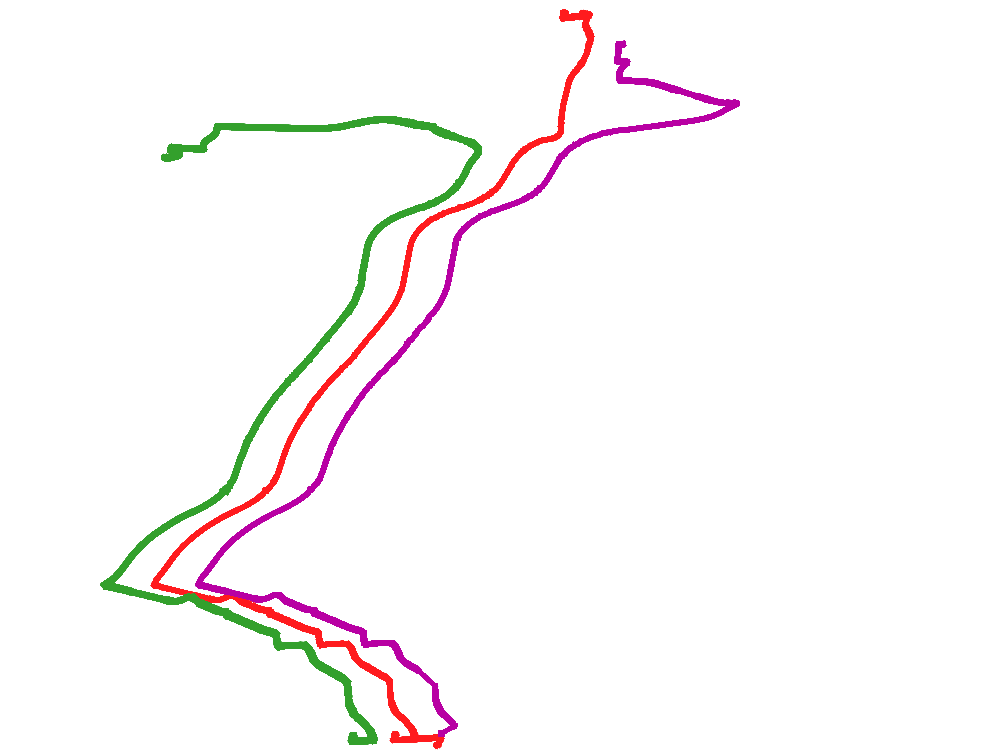
\includegraphics[width=80mm]{Pictures/LongTrips.png}
    \caption{Green, red and purple route for experiment 2}
    \label{fig:longtrips}
\end{figure}

This test case is a three-way comparison and the routes are not exactly the same, although they share a majority of the same segments, as seen in figure \ref{fig:longtrips}. Looking at Table \ref{tab:longtrips}, the differences in metrics are very clear. Green trip is driven extremely well compared to the other two; low counts on accelerations, brakes and jerks, and intervals exclusively in the low end, and almost no speeding. Note that the total counts on this trip are about as low as the trips in test case 1 (See table \ref{tab:shorttrips}), despite being approximately 4 times as long.
Looking at red trip for comparison, we have a vast increase in all counts; More accelerations, brakes and jerks, and worse distribution of the intervals. A total of 31.76 kilometers driven, 13.06 kilometers of these were driven above the speed limit, mostly in the interval of 20-30\% above the speed limit.

Note that despite of the massive differences in metrics, both of these trips were driven by the same car. Whether this indicates the driver being in a rush on green trip, or a different driver is difficult to predict with single examples - but the differences are clear.

The purple trip is as mentioned driven by a different car. Looking at acceleration, brake and jerk counts along with the amount of speeding in table \ref{tab:longtrips}, the trip is clearly positioned between the other two trips. The matching intervals provides an extended view on these counts, indicating that this driver consistently makes rapid changes in speed. Both acceleration, brake and jerk intervals reached higher values than 11 on several occasions. The worst offender is the jerks distribution - 56\% of the jerks is positioned in the worst interval 11$m/s^3$ or above that. This is a striking contrast to the green and red trip, in which the worst case for this interval is 8\% on braking.

The aggregated scores seen in \ref{tab:longtripscores} are as expected given the driving patterns. Red trip is very expensive due to the excessive speeding, and the sheer amount of changes in speed. Green trip comes very close to the best possible score of 32764.82(base $+$ roadtype) for a route of 32043.83 meters. The extra cost from driving style adds up to only 825.57 meters(all metrics). Purple trip is charged extra for driving on a Tuesday morning where heavier traffic is expected. In spite of red trip having higher counts of accelerations brakes and jerks in total amounts, purple trip cost more on these points combined. This is due to the distributions which were significantly worse for the purple trip, meaning each delinquency has been significantly more severe.

\begin{table}
    \centering
    \begin{tabular}{llll}
    \textbf{Score type} & \textbf{Green trip} & \textbf{Red trip} & \textbf{Purple trip}\\ \hline
    Base                & 32043,83            & 31763,97          & 31660,97            \\
    RoadType            & 720,99              & 873,51            & 696,54              \\
    Critical time       & 0                   & 0                 & 237,46              \\
    Speeding            & 8,96                & 12291,53          & 2544,64             \\
    Acceleration        & 115,16              & 431,74            & 914,66              \\
    Brake               & 317,33              & 1996,90           & 1778,41             \\
    Jerk                & 384,12              & 998,09            & 2857,83             \\ \hline
    \textbf{Total}      & \textbf{33590,39}   & \textbf{48355,73} & \textbf{40690,52}   \\ \hline
    \end{tabular}
    \caption{Trip score distribution for test case 2}
    \label{tab:longtripscores}
\end{table}

\begin{table*}
    \centering
    \begin{tabular}{>{\bfseries}l|ll|}
    Figure color             & Green               & Red                 \\
    Car ID                   & 16                  & 16                  \\
    Weekday                  & Thursday            & Thursday            \\
    Start                    & 18:35:59            & 19:02:22            \\
    End                      & 18:44:15            & 19:11:24            \\
    Distance (km)            & 8.08                & 8.07                \\
    Distance sped (km)       & 3.24                & 1.02                \\
    Accelerations ($>$5m/s)  & 23                  & 21                  \\
    Brakes ($>$5m/s)         & 40                  & 38                  \\
    Jerks ($>$5m/s)          & 15                  & 14                  \\
    Roadtype intervals       & 0 0 0 88 0 0 0 0    & 0 0 0 93 0 0 2 0    \\
    Speeding intervals       & 56 41 2 2 0 0 0 0   & 62 28 5 5 0 0 0 0   \\
    Acceleration intervals   & 0 0 87 0 4 9 0 0    & 0 0 67 10 24 0 0 0  \\
    Brake intervals          & 0 0 48 20 18 10 5 0 & 0 0 50 24 16 11 0 0 \\
    Jerk intervals           & 0 0 60 20 13 7 0 0  & 0 0 71 14 14 0 0 0  \\
    \end{tabular}
    \caption{Trip data for test case 1}
    \label{tab:shorttrips}
\end{table*}

\begin{table*}
    \centering
    \begin{tabular}{>{\bfseries}l|lll|}
    Figure color            & Green                & Red                 & Purple             \\
    Car ID                  & 10                   & 10                  & 14                 \\
    Weekday                 & Friday               & Sunday              & Tuesday            \\
    Start                   & 22:42:35             & 18:56:50            & 08:56:15           \\
    End                     & 23:11:42             & 19:23:45            & 09:29:19           \\
    Distance (km)           & 32.04                & 31.76               & 31.67              \\
    Distance sped (km)      & 0.02                 & 13.06               & 3.63               \\
    Accelerations ($>$5m/s) & 16                   & 49                  & 34                 \\
    Brakes ($>$5m/s)        & 29                   & 71                  & 55                 \\
    Jerks ($>$5m/s)         & 21                   & 56                  & 41                 \\
    Roadtype intervals      & 49 10 00 27 5  0 2 0 & 54 0 0 29 7 0 3 0   & 58 0 0 30 3 0 2 0  \\
    Speeding intervals      & 100 0 0 0 0 0 0 0    & 02 29 62 06 0 0 0 0 & 78 5 4 13 0 0 0 0  \\
    Acceleration intervals  & 0 0 94 6 0 0 0 0     & 0 0 84 6 8 2 0 0    & 0 0 68 3 6 0 3 21  \\
    Brake intervals         & 0 0 90 10 0 0 0 0    & 0 0 61 13 10 6 3 8  & 0 0 62 11 5 9 0 13 \\
    Jerk intervals          & 0 0 57 24 10 5 0 5   & 0 0 64 16 7 7 4 2   & 0 0 32 5 5 2 0 56  \\
    \end{tabular}
    \caption{Trip data for test case 2}
    \label{tab:longtrips}
\end{table*}

\input{Content/Conclusion/Conclusion}

%%%%%%%%%%%%%%%%%%%%%%%%%%%%%%%%%%%%%%%%%%%%%%%%%%%%%%%%%%%%%%%%%%%%%%%%%%%%%%%%

\section*{APPENDIX}

Appendixes should appear before the acknowledgment.

\section*{ACKNOWLEDGMENT}

The authors thanks Kristian Torp for his supervision and value input to the work behind this paper.


%%%%%%%%%%%%%%%%%%%%%%%%%%%%%%%%%%%%%%%%%%%%%%%%%%%%%%%%%%%%%%%%%%%%%%%%%%%%%%%%



\bibliographystyle{chicago}
\bibliography{Litterature/litteratur}


\end{document}
